\begin{figure}[h]
  \begin{center}
    \begin{tabular}{ccc}
      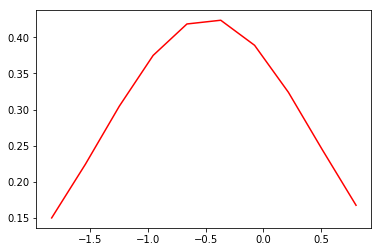
\includegraphics[width=0.32\hsize]{figure/10__1.png} &
      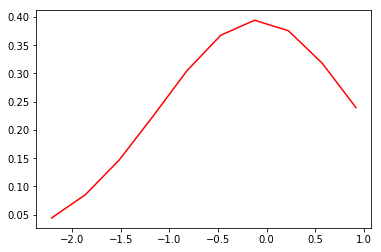
\includegraphics[width=0.32\hsize]{figure/10__2.png} &
      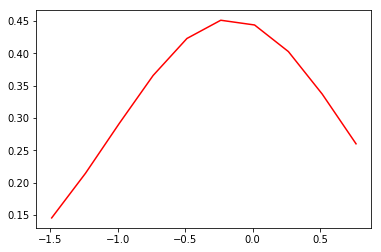
\includegraphics[width=0.32\hsize]{figure/10__3.png} \\
      試行1 & 試行2 &試行3
    \end{tabular}
    \caption{標準正規分布に基づく10個の乱数の分布}
    \label{figure1}
  \end{center}
\end{figure}
\begin{figure}[h]
  \begin{center}
    \begin{tabular}{ccc}
      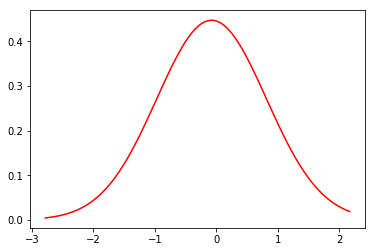
\includegraphics[width=0.32\hsize]{figure/100__1.png} &
      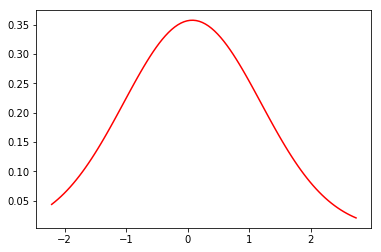
\includegraphics[width=0.32\hsize]{figure/100__2.png} &
      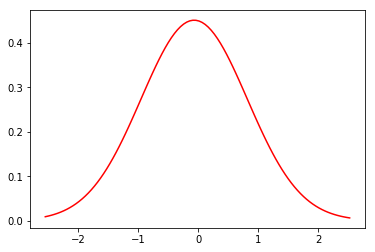
\includegraphics[width=0.32\hsize]{figure/100__3.png} \\
      試行1 & 試行2 &試行3
    \end{tabular}
    \caption{標準正規分布に基づく100個の乱数の分布}
    \label{figure1}
  \end{center}
\end{figure}
\begin{figure}[h]
  \begin{center}
    \begin{tabular}{ccc}
      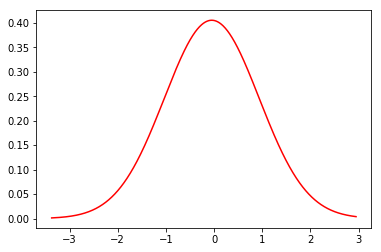
\includegraphics[width=0.32\hsize]{figure/1000__1.png} &
      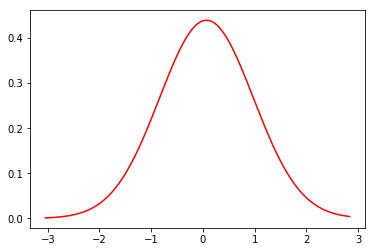
\includegraphics[width=0.32\hsize]{figure/1000__2.png} &
      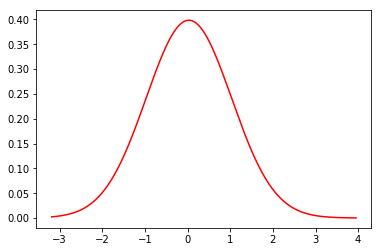
\includegraphics[width=0.32\hsize]{figure/1000__3.png} \\
      試行1 & 試行2 &試行3
    \end{tabular}
    \caption{標準正規分布に基づく1000個の乱数の分布}
    \label{figure1}
  \end{center}
\end{figure}
\begin{figure}[h]
  \begin{center}
    \begin{tabular}{ccc}
      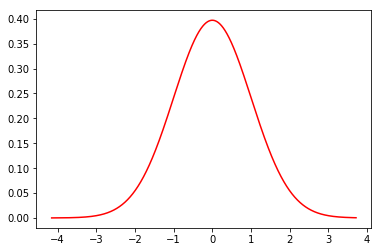
\includegraphics[width=0.32\hsize]{figure/10000__1.png} &
      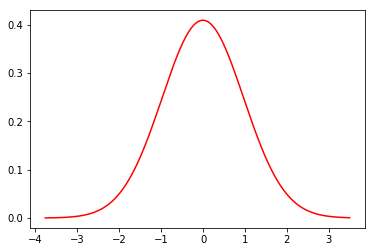
\includegraphics[width=0.32\hsize]{figure/10000__2.png} &
      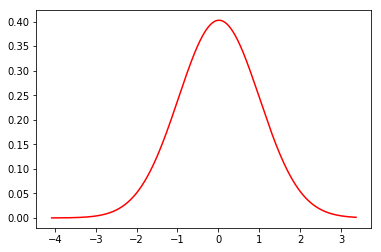
\includegraphics[width=0.32\hsize]{figure/10000__3.png} \\
      試行1 & 試行2 &試行3
    \end{tabular}
    \caption{標準正規分布に基づく10000個の乱数の分布}
    \label{figure1}
  \end{center}
\end{figure}
